\documentclass[letterpaper, 11pt]{article}
%\usepackage[round]{natbib}

\usepackage{mathtools}
\usepackage{setspace} 
\usepackage{dsfont}
\usepackage{amsfonts}
\usepackage{amsmath}
\usepackage{subcaption}
\usepackage{paralist}
%\usepackage{subfig}
\usepackage{times}
\usepackage{latexsym}
\usepackage{graphicx}
\usepackage[T1]{fontenc}
\usepackage{tikz}
\usepackage{url}
\usepackage{pgfplotstable}
\usepackage{titlesec}
\usepackage{color}
\usepackage{lipsum,adjustbox}
\usepackage[font={small}]{caption}
\usetikzlibrary{positioning}
\usepackage{bbm}

\makeatletter
\newcommand{\@BIBLABEL}{\@emptybiblabel}
\newcommand{\@emptybiblabel}[1]{}
%\makeatother
\usepackage[hidelinks]{hyperref}


\usepackage{acl2012}
\graphicspath{{./plots/}}
\newcommand{\com}[1]{}
%\newcommand{\oa}[1]{}
%\newcommand{\lc}[1]{}
\newcommand{\oa}[1]{\footnote{\color{red}OA: #1}}
\newcommand{\oamod}[1]{{\color{red}#1}}
\newcommand{\lc}[1]{\footnote{\color{blue}LC: #1}}


\newenvironment{myequation}{
  \vspace{-1em}
 \begin{equation}
}{
 \end{equation}
 \vspace{-1.2em}
}
\newenvironment{myequation*}{
	\vspace{-1em}
	\begin{equation*}
}{
\end{equation*}
\vspace{-1.2em}
}


\begin{document}

\title{Conservatism and Over-conservatism in Grammatical Error Correction}
%\author{
%  Leshem Choshen\textsuperscript{1} and Omri Abend\textsuperscript{2} \\
%  \textsuperscript{1}School of Computer Science and Engineering,
%  \textsuperscript{2} Department of Cognitive Sciences \\
%  The Hebrew University of Jerusalem \\
%  \texttt{leshem.choshen@mail.huji.ac.il, oabend@cs.huji.ac.il}\\
%}
\maketitle

\begin{abstract}
  %Evaluation in Grammatical Error Correction (GEC) is generally carried out
  %by comparison to references. Previous work discussed the necessary low
  %  coverage of such protocols given the multitude of different ways to correct a sentence,
  %and proposed 
  %In this paper we discuss the impact of using 
  %discusses the implications of such reference-based evaluation on
  Grammatical Error Correction systems (henceforth, {\it correctors}) aim to correct ungrammatical text,
  while changing it as little as possible. However, whereas such conservatism is a virtue for correctors,
  we find that state-of-the-art systems make substantially less changes to the source sentences than needed.
  Analyzing the distribution of possible corrections for a given sentence,   
  we show that this over-conservatism likely stems from
  the inability of a handful of reference corrections to account for the full variation of valid
  corrections for a given sentence. This results in undue penalization of valid corrections,
  thus disincentivizing correctors to make changes.
  We also show that simply increasing the number of references is unlikely to resolve this problem,
  and conclude by presenting an alternative reference-less approach based on semantic similarity.
  %one by , and the other by using semantic evaluation.
  %Does grammatical error correction systems learn not to learn?
  %We show that state-of-the-art systems are over conservative and are reluctant to correct. We analyze the distributions of
  % corrections showing that a single ungrammatical sentence tends to have hundreds of valid corrections, a problem for
  %current evaluation methods which are based on a reference or two. We suspect it causes correctors to avoid correcting and proceed to analyze the effect of
  %increasing amount of references in the gold standard on different evaluation measures. Discovering that more references are helpful but only to a
  %certain point, we also find that semantic structures are promising as a measure that is not reference based.
\end{abstract}

\section{Introduction}

% Error correction 
% evaluation in error correction and its centrality
% faithfulness to the source meaning is important, and this has been noted but prev work, and evaluation is geared towards it
% gap in evaluation: however, steps taken to ensure conservativeness in fact push towards formal conservativism by their definition (theoretical claim about the measure)
% this may result in systems that make few changes. indeed we find that this is the case (empirical claim about systems)
%
% we pursue two approaches to overcome this bias.
%
% 1. increasing the number of references. this has been proposed before and pursued with m=2, but no assessment of its sufficiency or its added value over m=1 has been made. In order to address this gap we first charachterize the distribution of possible corrections for a sentence. We leverage this characterization to characterize the distribution of the scores as a function of $m$, and consequently assess the biases introduced by taking $m=1,2$ as with previous approaches. 
% We find that taking these values of $m$ drammatically under-estimate the system scores. 
% We back our analysis of these biases with an analysis of the variance of these estimators.
% We analyze the two commonly used scores, the M2 score often used for evalauted, and the accuracy score commonly used in training.
%
% 2. we note that in fact the important factor is semantic conservativism and explore means to directly assess how semantically conservative systems here through the use of semantic annotation. 
% We use the UCCA scheme as a test case, motivated by HUME.
% First question: is it well-defined on learner language. it is.
% Second question: are corrections in fact semantically conservate? to show that, we need to verify that the corrections make few (if any) semantic changes. our results indicate that this is the case: we show that the corrections are similar in (UCCA) structure to the source.
%
% conclusion (not in intro): we tried to use semantic similarity to improve systems.
% this is difficult due to semantic conservatism. we expect this will be in issue once evaluation is improved.
% future work.
% also future work: use multiple references in training (did people do that?)
%
% sections:
% 1. Introduction
% 2. Formal conservativism in GEC
% 3. First approach: Multiple References
% 3.1. A Distribution of Corrections
% 3.2. Scores (M2, accuracy index, accuracy exact)
% 3.3. Data
% 3.4. Bias of the Scores (setup + results)
% 3.5. Variance of the Scores (setup + results)
% 4. Second approach: Semantic Similarity
% 4.1. Semantic Annotation of Learner Language (prev work)
% 4.2. UCCA Scheme (see HUME)
% 4.3. Similarity Measures (including prev work of elior)
% 4.4. Empirical Validation: IAA, semantic conservativism vs. gold std
% 5. Conclusion
%
% is a challenging research field, which interfaces with many
%other areas of linguistics and NLP. The field
Grammatical Error Correction (GEC) is receiving considerable
interest recently, notably through the GEC-HOO \cite{dale2011helping,dale2012hoo} and
CoNLL shared tasks \cite{kao2013conll,ng2014conll}.
Within GEC, considerable effort has been placed on evaluation
\cite{tetreault2008native,madnani2011they,felice2015towards,napoles2015ground},
a notoriously difficult challenge, in part due to the many valid corrections each learner's language (LL) sentence may
have \cite{chodorow2012problems}.

An important criterion in the evaluation of correctors
is their ability to generate corrections that are faithful to meaning of the source.
In fact, many would prefer a somewhat cumbersome or even an occasionally ungrammatical
correction over a correction that alters the meaning of the source \cite{brockett2006correcting}.
As a result, 
annotators are often instructed to be conservative in their corrections
when compiling gold standard corrections for the task
(e.g., in the Treebank of Learner English \cite{nicholls2003cambridge}).
There were different attempts to formally capture this precision/recall asymmetry such as the standardized use of $F_{0.5}$ over $F_{1}$ \cite{dahlmeier2012better} and the choices of weights in I-measure \cite{felice2015towards}.

However, during development and training penalizing over-correction more harshly than under-correction may lead to reluctance of correctors to
make any changes (henceforth, {\it over-conservatism}).
Using only one or two reference corrections, a common practice in GEC,
compounds this problem, as correctors are not only harshly penalized for making incorrect changes,
but are often penalized for making {\bf correct} changes not found in the reference.

Indeed, we show that current state of the art systems suffer from over-conservatism.
Evaluating the output of 12 recent correctors, we find that all of them
substantially under-predict corrections relative to the gold standard (\S \ref{sec:formal_conservatism}).

We first assess whether the undue penalization of valid corrections can be resolved by increasing the number
of references, which we denote with $M$ (\S \ref{sec:increase-reference}).
We start by estimating the number and frequency distribution of the valid corrections per sentence,
arriving at an estimate of over 1000 corrections for sentences of no more than 15 tokens.
We then consider two representative reference-based measures (henceforth, {\it RBMs}) for
assessing the validity of a proposed correction relative to a set of references, 
and characterize the distribution of their scores as a function of $M$. 
Our results show that both measures substantially under-estimate the true performance of
the correctors. Moreover, they show that increasing $M$ only partially addresses
the incurred bias, as both RBMs approach saturation for $M$ values of 10--20,
indicating that a prohibitively large $M$ may be required for reliable estimation.

Our findings echo the results of \newcite{bryant2015far}, who study the effect of $M$
on $F$-score, the most commonly used measure for GEC. Their work focused on
obtaining a more reliable estimate of correctors' performance, and proposed to do so
by normalizing corrector's estimated performance with the performance of a human corrector. However, while such normalization may yield more realistic performance estimates,
it has no effect on the training and tuning of correctors. 

We conclude by proposing an alternative reference-less semantic evaluation approach which assesses the extent to which
a correction faithfully represents the semantics of the source, by measuring the similarity of their semantic structures (\S \ref{sec:Semantics}).
This approach can be combined with a reference-less measure of grammaticality, based on automatic error detection, as
proposed by \newcite{napoles-sakaguchi-tetreault:2016:EMNLP2016}.
Our experiments support the feasibility of the proposed approach,
by showing that (1) semantic structural annotation can be consistently and automatically applied to LL, (2) that the proposed measure is less prone to unduly penalize valid corrections and (3) that the measure penalizes corrections that change the semantic structure significantly.

%
%
%We define a measure, using the UCCA scheme \cite{abend2013universal} as a
%test case, motivated by its recent use for machine translation
%evaluation \cite{birch2016hume}.
%We annotate a section of the NUCLE parallel corpus \cite{dahlmeier2013building},
%
%The two approaches address the insufficiency of using too few references from
%complementary angles. The first attempts to cover more of the probability
%mass of valid corrections by taking a larger $M$, 
%while the second uses semantic instead of string similarity, in order
%to abstract away from some of the formal variation between different valid corrections.
%
%%%%%%%%%%%%%%%%%%%%%%%%%%%%%%%%%%%%%%%%%%%%%%%%%%%%%%%%%%%%%%%%%%%%%%%%%%%%%%
\section{Over-Conservativism in GEC Systems}\label{sec:formal_conservatism}
%The field of GEC was always thriving or conservatism in its corrections, with the prominent example of using
%$F_{0.5}$ emphasizing precision over recall(\cite{ng2014conll}). we wish to highlight the problem that
%arises from pursuing this conservatism as done today.
%Then, we wished to be conservative, and we achieved that, why shouldn't we rejoice just yet? Theoretically, we might be progressing towards not correcting at all, instead of progressing towards correcting more accurately. 
%
%Manual analysis showed excessive formal conservatism and under correction.
%Albeit important, manual analysis is not enough and we aimed for generating some quantitative measures. 
%
We demonstrate that current correctors
suffer from over-conservatism: they tend to make too few changes to the source.
\subsection{Notation}
We assume each source sentence $x$ has a set of valid corrections $Correct_x$,
and a discrete distribution $\mathcal{D}_x$ over them, where $P_{\mathcal{D}_x}(y)$
for $y \in Correct_x$ is the probability a human annotator would correct $x$ as $y$.

Let $X$ be the evaluated set of source LL sentences where $X$ consists of the sentences $x_{1}\ldots x_N$, each independently sampled from some distribution $\mathcal{L}$ over LL sentences and denote $\mathcal{D}_{i}\coloneqq \mathcal{D}_{x_i}$.
Each $x_i$ is paired with $M$ corrections $Y_i = \left\{y_{i}^{1},\ldots, y_{i}^{M}\right\}$,
which are independently sampled from $\mathcal{D}_{i}$.\footnote{Our analysis assumes $M$
	is fixed across source sentences. Generalizing the analysis to sentence-dependent $M$
	values is straightforward.}
We define the {\it coverage} of $M$ references for a sentence $x_i$ to be
$P(y \in Y_i|y \in Correct_i)$ for $Y_i$ of size $M$, and $y$ sampled
according to $\mathcal{D}_i$.

A corrector $C$ is a function from LL sentences to proposed corrections (strings).
An assessment measure is a function from $X$, $Y$ and $C$ to
a real number. We use the term ``true measure'' to refer to the measure's output where the references include all possible corrections, i.e., $Y_i=Correct_i$ for every $i$.

\paragraph{Experimental Setup.}\label{par:experimental_setup}
We conduct all experiments on the NUCLE test dataset,
a parallel corpus of LL essays and their corrected versions,
which is the de facto standard in GEC.
The corpus contains 1414 essays in LL and 50 test essays, each of about 500 words.

We evaluate all participating systems in the CoNLL 2014 shared task,
in addition to three of the best performing systems on this dataset, a hybrid corrector, a phrase based machine translator and a neural network based corrector.
The particiapting systems and their abbreviations are: Adam Mickiewicz University (AMU),
University of Cambridge (CAMB), Columbia University and the University of Illinois at Urbana-Champaign (CUUI),
Indian Institute of Technology, Bombay (IITB), Instituto Politecnico Nacional (IPN),
National Tsing Hua University (NTHU), Peking University (PKU), Pohang University of Science and Technology (POST),
Research Institute for Artificial Intelligence, Romanian Academy (RAC), Shanghai Jiao Tong University (SJTU),
University of Franche Comt\'{e} (UFC), University of Macau (UMC), \newcite[RoRo]{rozovskaya2016grammatical}, \newcite[JMGR]{junczysdowmunt-grundkiewicz:2016:EMNLP2016} \newcite[char]{xie2016neural}.
All are trained and tested on the NUCLE corpus.

We compare the prevalence of changes made to the source by the correctors,
relative to their prevalence in the NUCLE reference.
In order to focus on the more substantial changes, we exclude from our evaluation


\paragraph{Measures of Conservatism.}
We consider three types of divergences between the source and the reference.
First, we measure to what extent \emph{words} were changed: altered, deleted or added.
To do so, we compute word alignment between the source and the reference, casting it
as a weighted bipartite matching problem, between the source's words and the correction's. 
Edge weights are assigned to be the edit distances
between the tokens.
We note that aligning words in GEC is much simpler than in machine translation,
as most of the words are kept unchanged, deleted fully, added, or changed slightly.
Following word alignment, we define the {\sc WordChange} measure
as the number of unaligned words and aligned words that were changed in any way.

Second, we quantify word \emph{order} differences using
Spearman's $\rho$ between the order of the words in the source sentence,
and the order of their corresponding words in the correction according to the word alignment.
$\rho=0$ where the word order is uncorrelated, and $\rho=1$ where the orders exactly match. We report the average $\rho$ over all source sentences pairs. 

Third, we report how many source sentences were split and how many concatenated by the reference and the correctors.
\com{
\begin{figure}
  \centering
  \begin{subfigure}[]{0.4\textwidth}
  	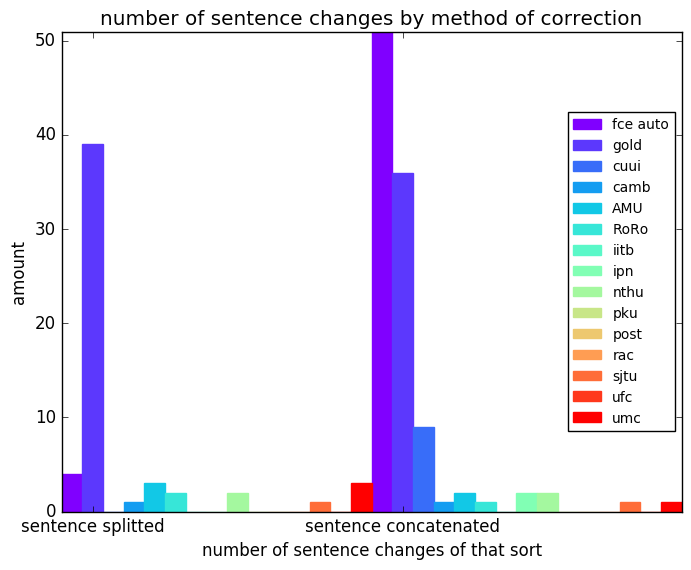
\includegraphics[width = \textwidth]{aligned}
  	\caption{Number of source sentences (y-axis) split 
  		(right bars) or concatenated (left bars) in the correction, according to the gold standard (striped column) and different correctors (colored columns). The gold standard makes about an order of magnitude more splits and concatenations than the correctors.\label{fig:split}}
  \end{subfigure}

  \begin{subfigure}[]{0.4\textwidth}
  	\com{\caption{\label{fig:rho}}}
    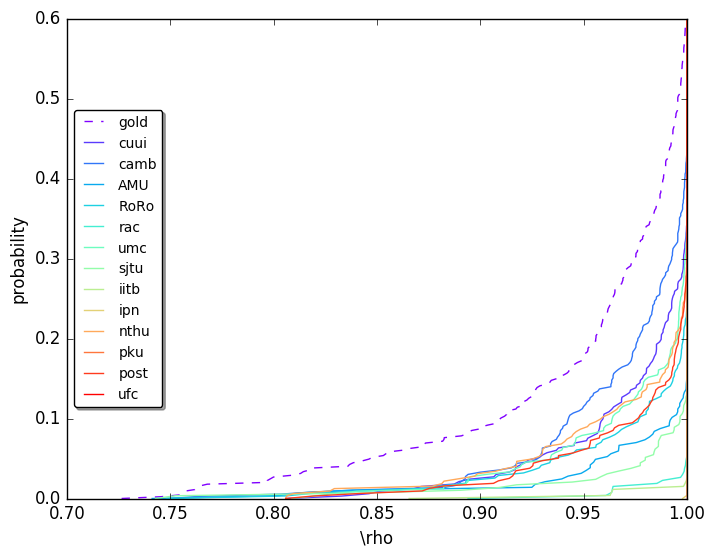
\includegraphics[width = \textwidth]{spearman_ecdf}
    \caption{Empirical cumulative probability (y-axis) of a sentence to get Spearman's rho values (x-axis) of word alignment. The gold standard(dotted line) makes word change alterations to more sentences than the correctors, and within these sentences, it changes order more substantially.\label{fig:rho}}
  \end{subfigure}

  \begin{subfigure}[]{0.4\textwidth}
  	%\caption{\label{fig:words_changed}}
  	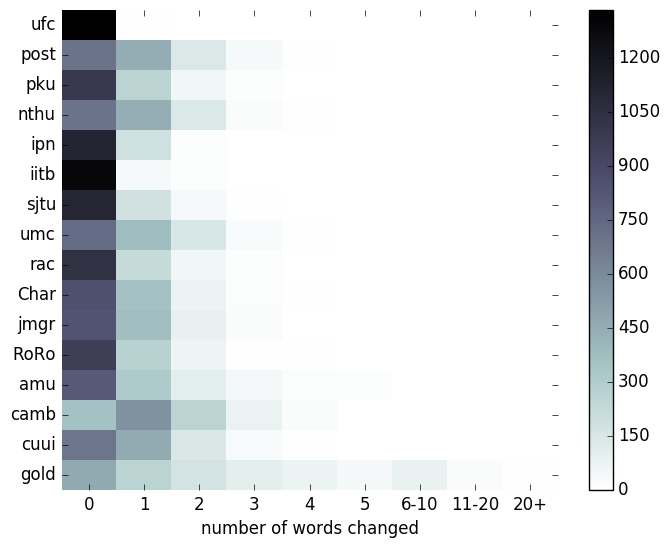
\includegraphics[width = \textwidth]{words_differences_heat}
  	\caption{Amount of sentences(heat) by number of words changed(x-axis) per system(y-label). The gold standard(bottom) corrects more words per sentences and more sentences relative to other systems.\label{fig:words_changed}}
  \end{subfigure}
  \com{\caption{(a) Number of source sentences (y-axis) split 
  		(right bars) or concatenated (left bars) in the correction, according to the gold standard (striped column) and different correctors (colored columns). The gold standard makes about an order of magnitude more splits and concatenations than the correctors.\\
  		(b) Empirical cumulative probability (y-axis) of a sentence to get Spearman's rho values (x-axis) of word alignment. The gold standard(dotted line) makes word change alterations to more sentences than the correctors, and within these sentences, it changes order more substantially.\\
  		(c) Amount of sentences(heat) by number of words changed(x-axis) per system(y-label). The gold standard(bottom) corrects more words per sentences and more sentences relative to other systems.\\
  		See \S\ref{par:experimental_setup} for a legend
  		of the systems.}\label{fig:over-conservatism}}
  \caption{\label{fig:over-conservatism}
    See \S\ref{par:experimental_setup} for a legend
    of the systems.}
  	\end{figure}
}
\begin{figure}
  \centering
  \begin{subfigure}[]{0.4\textwidth}
    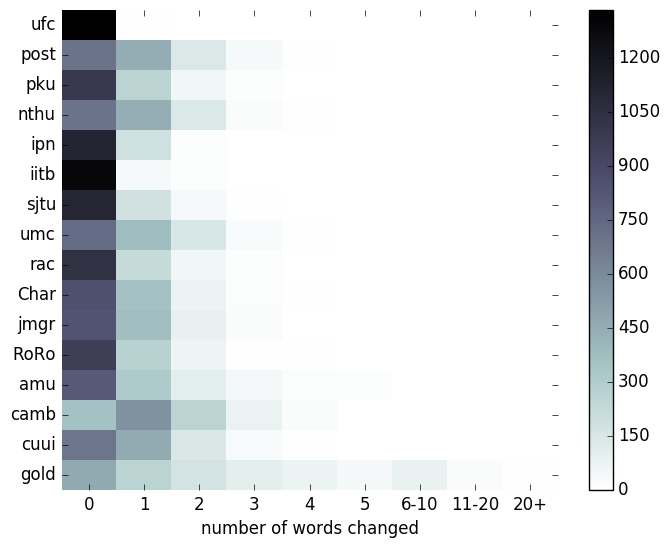
\includegraphics[width = \textwidth]{words_differences_heat}
  \end{subfigure}
  \begin{subfigure}[]{0.4\textwidth}
    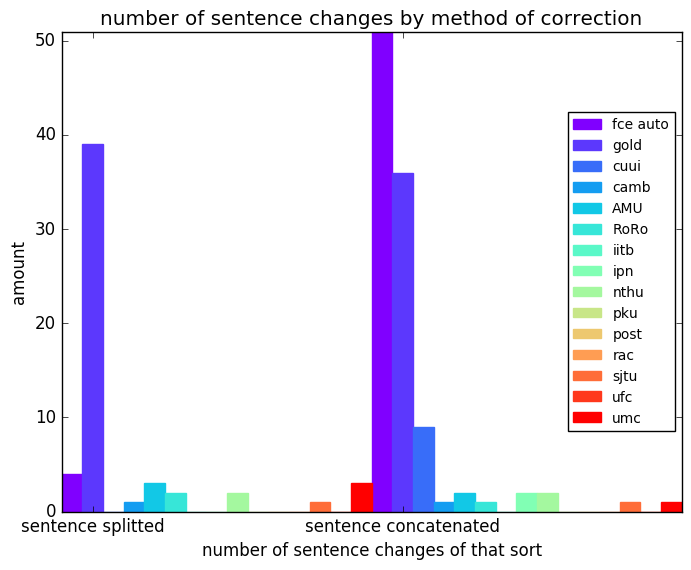
\includegraphics[width = \textwidth]{aligned}
  \end{subfigure}
  \begin{subfigure}[]{0.4\textwidth}
    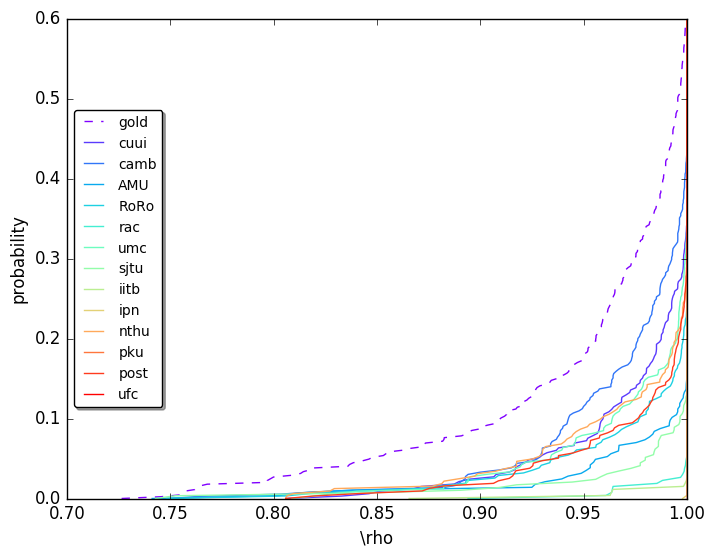
\includegraphics[width = \textwidth]{spearman_ecdf}
  \end{subfigure}
  \caption{\label{fig:over-conservatism}
    The prevalence of changes of different types in correctors' output and in the NUCLE references.
    The top figure presents the number of sentence pairs (heat) for each number of word changes
    (x-axis; measured by {\sc WordChange}) for each of the different systems and the references (y-axis).
    The middle figure presents the number of source sentences (y-axis) concatenated (right bars) or split (left bars) in the references (striped column) and in the correctors' output (colored columns).
    The bottom figure presents the percentage of sentence pairs (y-axis) where the
    Spearman $\rho$ values do not exceed a certain threshold (x-axis).
    See \S \ref{par:experimental_setup} for a legend of the correctors.
    The three figures show that under all measures, the gold standard references make
    substantially more changes to the source sentences than any of the correctors,
    in some cases an order of magnitude more.
  }
\end{figure}
\vspace{-.2cm}
\paragraph{Results.}
Figure \ref{fig:over-conservatism} presents the outcome of the three measures. 
%In \ref{fig:split} the amount of sentences each corrector has done is presented. In \ref{fig:words_changed} the accumulated sum of sentences by the words changed in each sentence of each of the correctors is presented. In \ref{fig:rho} the cumulative probability distribution of rho values out of all the sentences.
Results show that the reference corrections make changes to considerably more source sentences than any of the correctors, and within each changed sentence changes more words and makes more word order changes, often an order of magnitude more. For example, the reference has 36 sentences with 6 word changes, where the most sentences with 6 word changes by any corrector is 5.

For completeness, we measured the prevalence of changes in
another corpus, the TreeBank of Learner English \cite{yannakoudakis2011new}, and obtained similar results.
%While $89.6\%$ of NUCLE sentences need corrections,
%The prevalence of FCE consists only of ungrammatical sentences.
%As expected, FCE is a bit less conservative than NUCLE by our measures.
%
%
%%%%%%%%%%%%%%%%%%%%%%%%%%%%%%%%%%%%%%%%%%%%%%%%%%%%%%%%%%%%%%%%%%%%%%%%%%%%%%%%%%%%%
\vspace{-.1cm}
\section{Multi-Reference Measures}\label{sec:increase-reference}
%
In this section we argue that the observed over-conservatism of correctors likely stems
from them being developed to optimize RBMs that suffer from low-coverage.
We begin with a motivating analysis of the relation between low-coverage and over-conservatism (\S \ref{subsec:motivating_analysis}).We then continue with an empirical assessment of the distribution of corrections for a given sentence (\S \ref{subsec:corrections_distribution})
and the effect of $M$ on commonly used RBMs (\S \ref{subsec:Assessment-values}).
We discuss the implications of our results, concluding that RBMs may only partially address over-conservatism (\S \ref{subsec:mult_discussion}).
%
\vspace{-.2cm}
\subsection{Motivating Analysis}\label{subsec:motivating_analysis}
%
The relation between coverage and over-conservatism requires some explanation.
We abstract away from the details of the training procedure, and assume that correctors attempt to maximize an objective function, over some training or development data, and assume for simplicity of the argument that training proceeds by iterating over the samples, as with the Perceptron algorithm.

Assume the corrector is faced with a phrase which it predicts to be ungrammatical. Assume $p_{detect}$ is the probability that this prediction is correct.
Assume $p_{correct}$ is the probability it is able to predict
a valid correction for this phrase (including correctly identifying it as erroneous).
Finally, assume that the corrector is evaluated
against $M$ references for which the coverage of the phrase is $p_{coverage}$,
namely the probability that
a valid correction will be found among $M$ randomly sampled references.

We will now assume that the corrector may either choose to correct with the correction it finds the most likely or not at all. If it chose not to correct, its probability of being rewarded (i.e., its output is in the reference set $Y$) is $(1-p_{detect})$. Otherwise, its probability
of being rewarded is $p_{correct} \cdot p_{coverage}$.
In cases where

\vspace{.1cm}
\begin{small}
\begin{myequation}
  \label{eq:reward}
  p_{correct} \cdot p_{coverage} < 1-p_{detect} 
\end{myequation}
\vspace{-.1cm}
\end{small}

a corrector is disincentivized from altering the phrase.
We expect Condition \ref{eq:reward} to frequently hold in cases that
require non-trivial changes, which are characterized both by low $p_{coverage}$ (as non-trivial
changes can often be made in numerous ways), and by lower expected performance by the corrector.

Moreover, asymmetric measures (e.g., $F_{0.5}$) penalize invalidly correcting more
harshly than not correcting an ungrammatical sentence.
In these cases, Condition \ref{eq:reward} should be rephrased as

\begin{small}
	\vspace{-.1cm}
  \begin{myequation*}
    p_{correct} \cdot p_{coverage} - \left(1-p_{correct}p_{coverage}\right) \alpha < 1-p_{detect} 
  \end{myequation*}
  \vspace{-.1cm}
\end{small}

where $\alpha$ is the ratio between the penalty for introducing a wrong correction and the reward for a valid correction. Condition \ref{eq:reward} is much more likely to hold in these cases.

In order to validate this analysis empirically, we conduct an experiment for determining whether increasing
the number of references available for training indeed reduces conservatism. As there is no multiple-reference
corpus available which is large enough for re-training a corrector, we take an oracle reranking approach
as a simulation, and test whether the availability of increasingly more references to train on reduces
its conservativeness.

Concretely, given a set of sentences, each paired with $\mathcal{M}$ references, and given
a $k$-best list produced by a corrector, we define an oracle re-ranker that selects the highest
scoring correction of the $k$-best list, according to a given evaluation measure.
As a test case, we use the RoRo system, with $k$=100, and apply it to the 
largest available LL corpus which is paired with a substantial amount of references,
namely the NUCLE-test corpus, which has 12 references \cite{bryant2015far}. We use
the common F-score as an evaluation measure. 

We examine the conservativeness of the oracle reranker for different $M$ values, averaging
over 1312 samples of $M$ references from the available set of $\mathcal{M}=12$.
Our results show a consistent decrease in conservatism in
word changes with the increase in coverage (Figure \ref{fig:reranking_word_change}),
and no significant change in word order,\footnote{As we only rerank individual sentences,
  there is clearly no change in the number of sentences split or concatenated.}
indicating that conservatism is indeed related to the number of references available
to the learner.\footnote{We do not see a reason why this reduction in conservatism may
  a result of the setup in itself. In fact, oracle reranking may in some cases result
  in additional conservatism, as, as more references are used, some of them may be more
  similar to the source, thus increasing conservatism.}


%\com{Ideally, in order to validate this empirically, we should re-train correctors using multiple references, and re-examine their conservatism. However, corpora annotated with more than one correction are scarce. 
%As a proof of concept, we simulate a re-ranking procedure over the corpora of \newcite{bryant2015far}, which provide additional 10 references for each of sentence in the NUCLE test set. In order to abstract away from implementation details and from artefacts that may result from the small dataset available, we explore an oracle re-ranking setting, where the correction with the best Micro $F$-score taken from the 100-best list of the RoRo state-of-the-art corrector (see \S 2) is selected. The $F$-score is computed with varying numbers of references ($M$).}


\begin{figure}
	\vspace{-1em}
	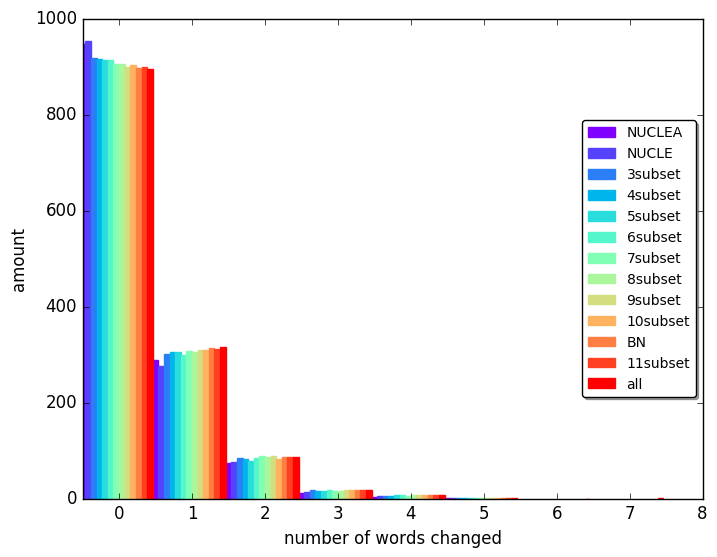
\includegraphics[width=8cm]{words_differences_hist_reranking}
	\caption{The amount of sentences (y-axis) with a given number of words changes (x-axis), following oracle reranking with different M values (column colors). 		\label{fig:reranking_word_change}
	}
	\vspace{-0.5cm}
\end{figure}

 \subsection{Data}
%
Our analysis assumes that we have a reliable estimate for the distribution of corrections
$\mathcal{D}_x$ for the source sentences we evaluate.
Our experiments in the following section are run on a random sample of 52 sentences with a
maximum length of 15 from the NUCLE test data.
Through the length restriction we avoid introducing too many independent
errors that may drastically increase the number of annotations variants (as every combination of corrections for these errors is possible), thus resulting in an unreliable estimation for $\mathcal{D}_x$.
Sentences with less than 6 words were discarded, as they were mostly a result of sentence segmentation errors.

Crowdsourcing has proven effective in GEC evaluation \cite{madnani2011they,napoles2015ground} and in
related tasks such as machine translation \cite{zaidan2011crowdsourcing,post2012constructing}. We thus
use crowdsourcing for obtaining a sample from $\mathcal{D}_x$. Specifically, for each of the 52 source
sentences, we elicited 50 corrections from Amazon Mechanical Turk workers.
%allowing for a reliable estimation of the distributions.
Aiming to judge grammaticality rather than fluency, we asked the workers to
correct only when necessary, not for styling.
4 sentences did not require any correction according to almost half the workers and were hence discarded.
%
\subsection{Estimating the Distribution of Corrections}\label{subsec:corrections_distribution}
%
We begin by estimating $\mathcal{D}_x$ for each sentence, using the crowdsourced corrections.
We use {\sc UnseenEst} \cite{zou2015quantifying}, a non-parametric algorithm that
estimates a multinomial distribution,
in which the individual values do not matter, only the distribution of probabilities
across values. {\sc UnseenEst} aims to minimize the ``earthmover distance''\oa{explain what this is or give a reference}
between the estimated histogram and the histogram of the distribution and has obtained excellent empirical
results in simulations.\footnote{An implementation of UnseenEst can be found in <to be disclosed upon publication>\com{\href{https://github.com/borgr/unseenest}}} 
{\sc UnseenEst} was originally developed for assessing how many
variants a gene might have, including undiscovered ones,
and their relative frequencies.
This is a similar setting to the one tackled here.
Our manual tests of {\sc UnseenEst} with small artificially created frequencies
showed satisfactory results.\footnote{All data we collected, along with the estimated
  distributions can be found in <to be disclosed upon publication>}

By the estimates from {\sc UnseenEst}, most source sentences have a large number of
corrections with low probability accounting for the bulk of the probability mass
and a rather small number of frequent corrections.
%The estimated distributions tend to have steps, with many corrections with the same (low) frequency.
Table \ref{tab:corrections_dist} presents the mean numbers of different corrections with frequency at least
$\gamma$ (for different values of $\gamma$), and their total probability mass.
For instance, 74.34 corrections account for 75\% of the total probability mass of the corrections, each
occurring with a frequency of 0.1\% or higher.

\begin{table}[h!]
	\vspace{-0.5cm}
  \centering
  \small
  \singlespacing
  \begin{tabular}{c|c|c|c|c|}
    %\cline{2-5} 
    & \multicolumn{4}{c|}{Frequency Threshold ($\gamma$)}\\ 
    %\cline{2-5} 
    & \multicolumn{1}{c}{0} & \multicolumn{1}{c}{0.001} & \multicolumn{1}{c}{0.01} & \multicolumn{1}{c|}{0.1}
    \\
    \hline
    Variants & 1351.24 & 74.34 & 8.72 & 1.35
    \\
    Mass & 1 & 0.75 & 0.58 & 0.37\\
    \hline
  \end{tabular}
  \caption{\label{tab:corrections_dist}
    Estimating the distribution of corrections $\mathcal{D}_x$.
    The table presents the mean number of corrections per sentence with probability of more than
    $\gamma$ (top row), as well as their total probability mass (bottom row).
  }
  \vspace{-0.3cm}
\end{table}

The overwhelming number of rare corrections raises the question whether these can be regarded as noise.
To test this we conducted another crowd-sourcing experiment, where 3 annotators were asked to
judge whether a correction produced in the first experiment, is indeed a valid correction. Results of the
mean number of annotators who judged a correction that was proposed a given number of times in the
training data, is given in Figure \ref{fig:accuracy_vals}. 
Results show that the original frequency of the correction has little effect on how often it was deemed
valid, where even the rarest corrections were judged valid 78\% of the times.

\begin{figure}[h!]
	\vspace{-.3cm}
	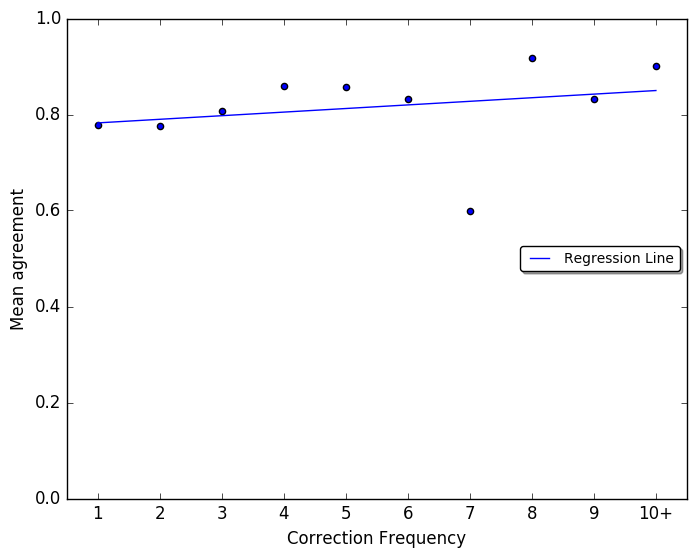
\includegraphics[width=8cm]{IAA_confirmation_frequency}
	\caption{The mean frequency ($y$-axis) in which a correction that was produced
          a given number of times ($x$-axis), was judged to be valid.
	} \label{fig:accuracy_vals}
	\vspace{-0.3cm}
\end{figure}

\subsection{Under-estimation as a function of M} \label{subsec:Assessment-values}
In the previous section we presented empirical assessment of the distribution of corrections to a sentence. We turn to estimate the resulting bias, i.e., the under-estimation of RBMs, for different $M$ values. 

We discuss two similarity measures. One is the sentence-level accuracy
(also called ``Exact Match'') and the other is the GEC $F$-score.

\paragraph{Sentence-level Accuracy.}
Sentence-level accuracy (also ``Exact Match'') is the percentage of corrections that
exactly match one of the references.
Accuracy is a basic, interpretable measure, used in GEC by, e.g. \newcite{rozovskaya2010annotating}.
It is also closely related to the 0-1 loss function commonly used
for training statistical correctors \cite{chodorow2012problems,rozovskaya2013joint}. 

Formally, given test sentences $X=\{x_1,\ldots,x_N\}$,
their references $Y_1,\ldots,Y_N$, and a corrector $C$,
we define $C$'s accuracy to be

\begin{small}
\vspace{-0.2cm}
  \centering
  \begin{myequation}\label{eq:acc_def}
    Acc\left(C;X,Y\right) = \frac{1}{N} \sum_{i=1}^N \mathds{1}_{C(x_i) \in Y_i}.
  \end{myequation}
\end{small}

Note that $C$'s accuracy is in fact an estimate of $C$'s probability to produce
a valid correction for a sentence, or $C$'s {\it true accuracy}. Formally:

 \begin{small}
   \centering
   \vspace{-0.2cm}
   \begin{myequation*}
     TrueAcc\left(C\right) = P_{x\sim{L}}\left(C\left(x\right)\in Correct_x\right).
   \end{myequation*}
   \vspace{-0.15cm}
 \end{small}
%
%We estimate $C$s quality by sampling a set of source sentences
%$x_1,\ldots,x_N \sim \mathcal{L}$, and evaluate the quality of $C(x_1),\ldots,C(x_N)$ relative
%to the source. 

The bias of $Acc\left(C;X,Y\right)$ for a sample of $N$ sentences, each paired with $M$ references
is then

\vspace{-0.6cm}
\begin{small}
  \centering
  \begin{flalign}
    &TrueAcc\left(C\right) - \mathbb{E}_{X,Y}\left[Acc\left(C;X,Y\right)\right] = &\\
    &TrueAcc\left(C\right) - P\left(C\left(x\right) \in Y\right)  = &\\
    &Pr\left(C\left(x\right) \in Correct_x\right)  \cdot &\\
    &\label{eq:bias} \left(1 - Pr\left(C\left(x\right) \in Y \vert C\left(x\right) \in Correct_x\right) \right) &
  \end{flalign}
\end{small}
\vspace{-1.5em}

We observe that the bias, denoted $b_M$, is not affected by $N$, only by $M$.
As $M$ grows, $Y$ approximates $Correct_x$ better, and $b_M$ tends to 0.

In order to gain insight into the evaluation measure and the GEC task
(and not the idiosyncrasies of specific systems), we consider an idealized learner,
which, when correct, produces a valid correction with the same
distribution as a human annotator (i.e., according to $\mathcal{D}_x$).
Formally, we assume that, if $C(x) \in Correct_x$ then $C(x) \sim \mathcal{D}_x$.
Hence the bias $b_M$ (Equation \ref{eq:bias}) can be re-written as

\begin{small}
	\vspace{-0.2cm}
\begin{myequation*}
  \centering
  P(C(x) \in Correct_x) \cdot (1 - P_{Y \sim \mathcal{D}_i^M,y\sim \mathcal{D}_x}(y \in Y)).
\end{myequation*}
\end{small}

We will henceforth assume that $C$ is perfect (i.e., its true accuracy $Pr\left(C(x) \in Correct_x\right)$ is 1).
Note that assuming any other value for $C$'s true accuracy
would simply scale $b_M$ by that accuracy.
Similarly, assuming only a fraction $p$ of the sentences require correction scales $b_M$ by $p$.
%
%Denote the bias of a perfect corrector with $b_M$. To recap:
%\begin{equation*}
%  b_M = 1 - P_{x \sim L, Y \in \mathcal{D}_x^M, y \sim \mathcal{D}_x}\left(y \in Y\right)
%\end{equation*}
%
%We turn to estimating $b_M$ empirically. We note that $Acc(C;X,Y)$
%is a sum of Bernoulli variables (i.e., a Poisson Binomial distribution), 
%with probabilities $p_i = P_{y \sim \mathcal{D}_i}\left(y \in Y_i\right)$.

We estimate $b_M$ empirically using its empirical mean on our experimental corpus:

\begin{small}
	\vspace{-1em}
  \begin{myequation*}
    \hat{b}_M = 1 - \frac{1}{N}\sum_{i=1}^N P_{Y \sim \mathcal{D}_i^M, y \sim \mathcal{D}_i}\left(y \in Y\right).
  \end{myequation*}
\end{small}

Using the {\sc UnseenEst} estimations of $\mathcal{D}_i$, we can compute $\hat{b}_M$
for any size of $Y_i$ (value of $M$). 
However, as this is highly computationally demanding, we estimate it using
sampling. Specifically, for every $M = 1,...,20$ and $x_i$, we sample $Y_i$ 1000 times
(with replacement), and estimate $P\left(y \in Y_i\right)$ as the covered probability mass
$P_{\mathcal{D}_i}\{y: y \in Y_i\}$.

We repeated all our experiments where $Y_i$ is sampled without replacement,
in order to simulate a case where reference corrections are collected by a single
annotator, and are thus not repeated. We find similar trends with faster increase
in accuracy reaching over $0.47$ with $M=10$.

%
%The resulting estimates for $p_i$ 
%define the estimate for the distribution of $Acc(C;X,Y)$.
%Given a set of LL sentences $x_1,...,x_N$ and their corresponding references
%$Y_1,...,Y_N$, we define the coverage of the reference set $Y_i$ for the sentence $x_i$ to be
%
%\begin{equation*}
%Cov\left(x_i,Y_i\right)=.
%\end{equation*}
%
%In order to gain insight into the accuracy measure, we need to know something about the distribution from which the given corrector chooses valid corrections. As each corrector might have its own biases, the most appealing choice would be to evaluate a corrector in which this distribution is the same as the one from which corrections for the gold standard are being drawn from. Formally, if $C\left(x_i\right) \in Correct_i$ then $C\left(x_i\right) \sim \mathcal{D}_i$. 
%
%Thus, the second term in Equation \ref{eq:correction-in-gs} is $p_i = \mathbb{E}_{Y_i}[Cov(x_i,Y_i)]$. 
%Therefore $Acc(C;X,Y)$ is distributed as
%a Poisson Binomial random variable (divided by $N$), with probabilities $\{p_i \cdot CP\}_{i=1}^N$. \footnote{A Poisson Binomial random 
%variable is a sum of Bernoulli variables with different success probabilities.} We also assume our corrector is always 
%correct (so $CP=1$), but as noted earlier any other value for $CP$ would only scale the results by $CP$.

\begin{figure}
	\vspace{-1em}
  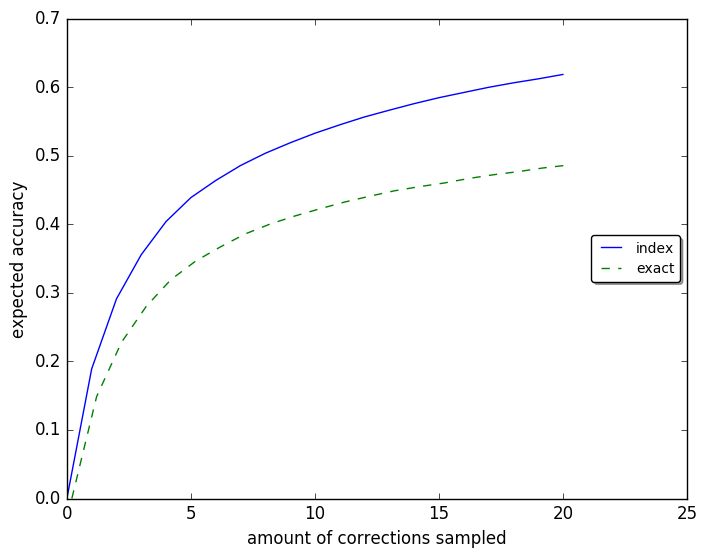
\includegraphics[width=8cm]{noSig_repeat_1000_accuracy}
  \caption{Accuracy and Exact Index Match values for a perfect corrector (y-axis)
    as a function of the number of references $M$ (x-axis).
    %Each data point is paired with a confidence interval ($p=.95$).     
  } \label{fig:accuracy_vals}
  \vspace{-0.5cm}
\end{figure}

Figure \ref{fig:accuracy_vals} presents the expected accuracy values for our perfect
corrector (i.e., 1-$\hat{b}_M$) for different values of $M$. 
Results show that even for values of $M$ which are much larger than those considered in the GEC literature (e.g., $M=20$),
the expected accuracy is only about 0.5. As $M$ increases, the contribution of each additional correction
  gets smaller to the point it contributes little to the accuracy (the slope is about 0.004 around $M=20$).

We also experiment with a more relaxed measure, {\it Exact Index Match}, which is only sensitive
to the identity of the changed words and not to what they were changed to. 
Formally, two corrections $c$ and $c'$ over a source sentence $x$ match
if for their word alignments with the source (computed as above) $a:\{1,...,\left|x\right|\} \rightarrow \{1,...,\left|c\right|,Null\}$
and $a':\{1,...,\left|x\right|\} \rightarrow \{1,...,\left|c'\right|,Null\}$, it holds that $c_{a\left(i\right)} \neq x_{i}$ iff $c'_{a'\left(i\right)} \neq x_{i}$, where $c_{Null}=c'_{Null}$.

Figure \ref{fig:accuracy_vals} also presents the expected accuracy in this case
for different values of $M$, which indicate that while scores of a perfect corrector are somewhat higher,
still with $M=10$, it is 0.54.
As Exact Index Match can be interpreted as an accuracy measure for error detection (rather than correction),
our results indicate that error detection systems may suffer from similar difficulties.
%
%{\color{red}Finally, Figure \ref{fig:accuracy_vals} include confidence intervals ($p=.95$), which are computed analytically. }
%\lc{I need to take what I said back.  is indeed used for the PDF, but currently we don't publish anything that uses the pdf. We do compute the confidence intervals, but those are intervals of the mean, for the graph. The account for the significance of the means we got i.e. for the choices of different sentences which we can't compute analytically. So we bootstrap again. The variance (not specifically significance) of the estimator was originally discussed with the analytical formula ($\sum_{i=1}^{N}P_{\mathcal{D}_x}(y_i \in Y)\cdot\left(1-P_{\mathcal{D}_x}(y_i \in Y)\right)$) when what is interesting is actually just that it decreases with N and when M gets away from 0.5.
%We can also compute using bootstrapping with 10000 repetitions }

The analytic tools we have developed support the computation of the entire distribution of the accuracy,
and not only its expected values. From Equation \ref{eq:acc_def} we see that Accuracy has a Poisson Binominal distribution (i.e., it is a sum of independent Bernoulli variables with different success probabilities), whose success probabilities are $P_{y,Y \sim \mathcal{D}_i}(y \in Y)$, which can be computed, as before, using {\sc UnseenEst}'s estimate for $\mathcal{D}_i$. Estimating the density function allows for the straightforward definition of significance tests for the measure, and can be performed efficiently \cite{hong2013computing}.\footnote{An implementation of this method and the estimated density functions will be released upon publication.}

\paragraph{$F$-Score.}
While accuracy is commonly used as a loss function for training GEC systems,
the $F_\alpha$ score is standard when reporting system performance (and consequently in hyper-parameter
tuning).

Computing $F$-score for GEC is not at all straightforward.
The score is computed in terms of {\it edit} matches between a correction and the references,
where edits are sub-strings of the source that are replaced in the correction/reference.
The HOO shared task used an earlier version of $F$-score, which required that the proposed corrections include edits explicitly.
Later on, relieving correctors from the need to produce edits, $F$-score was redefined optimistically, maximizing
over all possible annotations that generate the correction from the source.\footnote{Since our crowdsourced corrections
	do not include an explicit annotation of edits, we produce edits heuristically.}
$M^2$ \cite{dahlmeier2012better} was designated to compute this $F$ score and is the standard evaluation for GEC.

The complexity of the measure prohibits an analytic approach, and
we instead use a bootstrapping approach to estimate the bias incurred
by not being able to exhaustively enumerate the set of valid corrections.
%In short, bootstrapping methods sample with repetition from the empirical
%distribution of the observed data to estimate properties (e.g. confidence-interval)
%of the statistic (e.g. $F$-score) over the distribution. 
As with accuracy,
in order to avoid confounding our results with system-specific biases,
we assume the evaluated corrector is perfect and sample its corrections from the human distribution of corrections $\mathcal{D}_x$.

Concretely, given a value for $M$ and for $N$, we uniformly sample from our experimental
corpus source sentences $x_1,...,x_N$, and $M$ corrections for each $Y_1,...,Y_N$ (with replacement).
Setting a realistic value for $N$ in our experiments is important
for obtaining comparable results to those obtained on the NUCLE corpus (see below), 
as the expected value of $F$-score may depend on $N$ (unlike Accuracy, it is not additive).
In accordance with the NUCLE's test set,
we set $N=1312$ and assume that 136 of the sentences require no correction.
The latter reduces the overall bias by their frequency in the corpus,
and are thus important to include for obtaining realistic results.

The bootstrapping procedure is carried out by the
accelerated bootstrap procedure \cite{efron1987better}, with 1000 iterations.
We also report confidence intervals ($p=.95$), computed using the same procedure.\footnote{We
  use the Python scikits.bootstrap implementation.}
%
%For each sentence which had at least one error according to the NUCLE gold standard
%we sample $M$ sentences uniformly from the
%gathered empirical data to replace it. We leave sentences that do not need
%corrections untouched. This results in reference texts accounting for the
%variability in different choices of corrections while approximating the reduction of variability
%of a big $N$ by consisting of $N$ sentences overall.

% our results
Figure \ref{fig:F_Ms} presents the results of this procedure, which
further indicate the insufficiency of commonly used $M$ values for training and development (1 or 2)
for obtaining a reliable estimation of a corrector's performance.
For instance, the $F_{0.5}$ score for our perfect corrector, whose true $F$-score is 1,
is only 0.42 with $M=2$.
Moreover, the saturation effect observed for accuracy is even more
pronounced with our experiments on $F$-score.

The F-score coverage experiment is very similar to that of \newcite{bryant2015far},
who also compared the $F$-score of a human correction against an increasing number of references,
and indeed produced similar results \newcite{bryant2015far}.
They differ from the experiments reported in this section, in that
they did not attempt to estimate the distribution of corrections, and focused exclusively on the F-score
measure.

%
%\paragraph{}
%While our experiments focus on the accuracy and $F$-score measures, we expect
%our results to generalize to other RBMs (see Section \ref{sec:prev_work}).

%%%%%%%%%%%%%%%%%%%%%%%%%%%%%%%%%%%%%%%%%%%%%%%%%%%%%%%%%%%%%%%%%
\subsection{Significance of Real-World Correctors}\label{sec:real_world}
The bootstrapping method for computing the significance of the $F$-score can also
be useful for assessing the significance of the differences in correctors' performance
reported in the literature.
We report results with the bootstrapping protocol (\S \ref{subsec:Assessment-values})
to compute the confidence interval of different correctors with the current NUCLE
test data ($M=2$).
\begin{figure}
  \includegraphics[width=8cm]{$F_{0.5}$_Ms_significance}
  \caption{
    $F_{0.5}$ values for a perfect corrector (y-axis) as a function of the number of references $M$ (x-axis).
    Each data point is paired with a confidence interval ($p=.95$).\label{fig:F_Ms}}
\vspace{-0.5cm}
\end{figure}

\begin{figure}
  \includegraphics[width=8cm]{$F_{0.5}$_significance}
  \caption{$F_{0.5}$ values for different correctors, including confidence interval ($p=.95$).
    The left-most column (``source'') presents the $F$-score of a corrector that doesn't make any
    changes to the source sentences.
    See \S \ref{par:experimental_setup} for a legend of the correctors.\label{fig:F_correctors}}
\vspace{-0.5cm}
\end{figure}

Our results (Figure \ref{fig:F_correctors}) present a mixed picture: some
of the differences between previously reported $F$-scores are indeed significant and some are not.
For example, the best performing corrector is significantly better than the second, but the latter
is not significantly better than the third and fourth.

%Nevertheless, it seems that $M=2$ value taken in NUCLE is sufficiently high
%to generally obtain statistically significant ranking of the different correctors.

\subsection{Discussion}\label{subsec:mult_discussion}
% -- we saw that we have dramatic under-estimation
% -- but is this a problem? for instance, in the last section we saw we can get statistical significance between systems by increasing
%    N even with a low M
% -- balancing $N$ and $M$ is important;
%      other people have looked at similar things (not to re-label or not to re-label). we stress that
%      while for statistical significance increasing $N$ is sufficient, this would not solve this problem:
% -- low coverage entails other problems: it incentivizes systems not to correct, even if they can perfectly predict valid corrections.
% -- mathematical argument
% -- indeed, we see RoRo > Perfect and other systems are close to Perfect. it could be that they are better taylored to
%    those corrections produced by the NUCLE annotators. however in section 2 we saw that they are not.
%    we hypothesize that this is the reason.
%

Our empirical results show that the number of corrections needed for reliable reference-based measures may
be prohibitively large in practice.
Results suggest that there are hundreds of valid corrections with low probability, whose total probability mass
is substantial. RBMs such as accuracy and $F$-score thus show diminishing returns from increasing the value of $M$ over values of about 10.
%
%All these findings suggest that it is too costly to increase $M$ in development data to the extent asymmetric evaluation will not lead to over-conservatism. The exact index match analysis also suggests $M=1,2$ coverage is also low for detection. When detection is separate from correction this might result in over-conservatism. 
%
%about a quarter of the probability mass of valid corrections (\S \ref{subsec:Assessment-values}).
%
%The factors controlling significance are two. Variation across sentences themselves (different $D_x$)
%which is reduced with $N$ and the variation across choices of corrections which might be reduced with
%either $M$ or $N$. One can rightly deduce that large $N$ is sufficient for variation, but it will not
%solve the other problems: under-estimation of true performance,
%over-conservatism, possible issues when training systems, and might be more costly than annotating
%a larger $M$ without acquiring more sentences and also annotating them.
%Choosing how to balance is dependent on the goals of the one collecting data, and affects over
%the mean value as well, as discussed in \ref{subsec:Assessment-values}. Thus, we bring supporting data and
%leave the decision to the reader. 

Returning to condition (\ref{eq:reward}) (\S \ref{subsec:motivating_analysis}), we find that the coverage
(which is equal to the accuracy depicted in Figure \ref{fig:accuracy_vals})
is lower than 0.5 for $M=2$ on average (for short sentences). For cases of non-trivial
changes, we expect it might be even lower, suggesting that condition (\ref{eq:reward}) often
holds in practice, incentivizing over-conservatism.

Considering the $F$-score of the best performing systems in Figure \ref{fig:F_correctors}, and
comparing them to the $F$-score of a perfect corrector with $M=2$, we find that their scores are comparable,
where RoRo in fact surpasses a perfect corrector's $F$-score.
While it is possible that these correctors outperform the perfect corrector by learning how to
correct a sentence in the same way as one of the NUCLE annotators did, we view this possibility
as unlikely as our results (\S\ref{sec:formal_conservatism}) show that
the output of these systems considerably diverges from NUCLE's references.
A more likely possibility is that these systems' high performance relative to a perfect corrector's
is due to these correctors having learned to predict when not to correct.

Two recent RBMS have been proposed.
One is {\sc I-measure} \cite{felice2015towards}
which introduces novel features to GEC evaluation, such as distinguishing
different quality levels of ungrammatical corrections (e.g., some improve the quality of
the source, while others degrade it), and restricting edits to only consist of single words,
rather than phrases. The other is GLEU \cite{napoles2015ground}, an adaptation of BLEU that 
was shown to correlate well with human rankings. We expect our findings, that RBMs substantially under-estimate the
performance of correctors, to generalize to these RBMs, as they all
apply string similarity measures relative to a fairly small number of references.
These measures thus address orthogonal gaps in GEC evaluation from the ones presented here.
Following the proposal of \newcite{sakaguchi2016reassessing}, to emphasize fluency over grammaticality
in reference corrections, only compounds this problem, as it results in a larger number of valid corrections.

%Also, changing from grammatical corrections to fluency ones results in more possible corrections, and consequently a larger bias.

Finally, note that addressing under-estimation by comparing to
a human expected score (in our terms, a perfect corrector) with the same $M$ \cite{bryant2015far},
does not address over-conservatism, as it only
scales the original measure. Moreover, as seen above, a human correction's score
is not necessarily an upper bound, as an over-conservative corrector may surpass a perfect corrector in performance.

\com{
\subsection{Discussion}
{\color{red}\label{subsec:low_coverage_over_conservatism}
	\lc{in the introduction the order is in reverse, we first discuss and then we show this is indeed the case, is that a problem? It somehow seems more structured this way, after experiments and more fluent from a birds eye view to first reason why we check it anhe say it is true.}d t
	 The common practice of using one or two references in GEC evaluation yields a substantial under-estimation of system's performance using $F$-score \cite{bryant2015far} or other RBMs (\S\ref{sec:increase-reference}).
	 Theoretically this under estimation could lead to over-conservatism. In the case of detection, the reason is straightforward. If for a given type of error $t$ there is less than 50\% agreement in the gold standard about whether this should be detected as an error or not. Than a perfect corrector will not detect $t$ errors.
	 
	 The same holds for corrections, which we see is the case for a small $M$ \cite{bryant2015far}.
	 Importantly, low coverage of the reference set,
	 in conjunction with asymmetric evaluation measures that penalize over-correction
	 more severely than under-correction, result in evaluation measures that further incentivize correctors not to correct.
	 Assume that for a given source sentence $x$, references $Y \sim \mathcal{D}_x$, and proposed correction $c$,
	 a given evaluation measure increases by $\alpha$ if $c \in Y$, and decreases by $\beta > \alpha$ if $c \notin Y$.
	 %Assume that the corrector corrects with , i.e., it invariably produces $y \in Correct_x$.
	 If the covered probability mass $P(y \in Y)$ for $Y$ of size $M$ and $y$ sampled from $\mathcal{D}_x$
	 the expected utility of the corrector from producing $y$ is
	 \vspace{-0.8cm}
	 \begin{small}
	   \begin{center}
	     \begin{flalign*}
	 &P(y \in Y|y \in correct)P(y \in correct) \cdot \alpha - P(y \notin Y) \cdot \beta = &\\
	 &P(y \in Y|y \in correct)P(y \in correct) \cdot \alpha -&\\ &(P(y\notin correct) + P(y\in correct)P(y \notin Y)) \cdot \beta = &\\
	 &P(y \in Y|y \in correct)P(y \in correct) \cdot \alpha -&\\
	 &(1-P(y\in correct)P(y \in Y)) \cdot \beta = &\\
		   \end{flalign*}
	   \end{center}
	\end{small}
	\lc{I used the opposites (1-P) on the last step, how did you simplify it further?}
	For example (if we see in bryant probabillity X for that Y for that, etc. when we will be sure about the formula I will write it.)
	This implies that a corrector optimized in such circumstances will result in over-conservatism. We hypothesize this is a main reasons for the results shown in this section.}
}
%
 %we turn to discussing what values of $M$ yield a reliable estimate of the performance of GEC systems. While there is no one answer to this question, and coverage can be low even with $M$ values of 20, both measures we considered begin to plateau (in the case of $F$-score) or present linear increases after an initial concave behavior (in the case of accuracy) at $M$ values of 8--10. This may indicate that such values are a reasonable balance between cost and bias.
%
%Finally, there a few assumptions made in our experiments that are worth fleshing out.
%First, e.g. the explanation of a bad sampling is not probable but can not be refuted. We assume that the sentences we picked are a good representation of the overall sentences, but know they might be a bit simpler as we did not choose very long sentences for the reasons mentioned earlier. Another assumption is that the simple automatic edits are not a big shift in respect to the human edits.
%
% it could be that they are better taylored to
% those corrections produced by the NUCLE annotators. however in section 2 we saw that they are not.
% we hypothesize that this is the reason.
%
%An interesting finding comes from the combination of the scores of a perfect corrector with the scores correctors get (with $M=2$). Some correctors get a result close to the perfect score, with one actually surpassing it. If we consider the results from section \ref{sec:formal_conservatism} it is evident that they are far from being a perfect corrector, as many sentences which evidently need correcting (even if there is more than one way to correct) are not corrected by them. Then how can they get such a high score?
%
%
%The effect of under estimation on evaluation and hence on how correctors are perceived is obvious. 
%Perhaps less obvious will be how under estimation affects the development
%process. We shall consider any evaluation which scores a wrong correction lower than no correction at all
%(e.g. $F$-score). For simplicity lets consider a scenario with only one sentence. We denote by $r>0$ the
%reward for a valid correction, $pu>0$ the punishment for a wrong correction and 0 otherwise.
%Thus, an average the score of a correction $x$ would be
%$S\left(x\right) = p\left(x\in y\right)*r - \left(1-p\left(x\in y\right)\right)*pu$.
%Under the assumption that development cycles or ML is gradually optimizing to get closer to the best solution,
%we will examine an all knowing perfect corrector.
%This corrector may take into account the probabilities of corrections to be in the gold standard.
%When choosing to correct such a corrector will choose the most frequent correction yielding $max_xS\left(x\right)$.
%Notably, not matter what are $r, pu$ when $p\left(x\in y\right)$ is small enough the perfect
%corrector will choose \emph{not} to correct.
%
	
%To conclude the main discussion of this section, if the NLP community has agreed one correction is not enough\cite{tetreault2008native}
%%we can now say 2 is no magic number either. On both measures we see a large improvement in coverage when enlarging $M$, suggesting that a more reasonable $M$ to choose would be somewhere around 7 where the high probability corrections are probably covered and the graph turns semi-linear. The results also strongly support the hypothesis assessment values are very low, and hence might be a cause for over conservatism.
%Another conclusion to be made is that given a value from the assessment process we may estimate how low the value is in respect to the perfect assessment. Some may wish to correct for this under assessment.
%
%
%
%
%
%
%%%%%%%%%%%%%%%%%%%%%%%%%%%%%%%%%%%%%%%%%%%%%%%%%%%%%%%%%%%%%%%%%%%%%%%%%%%%%%%%%%%%%%
\section{Semantic Faithfulness Measure}\label{sec:Semantics}
%
%
%Conservatism is considered an important trait for a corrector, reflected for example
%in the selection of $F_{0.5}$, which emphasizes precision over recall, as the
%standard evaluation measure in GEC.
%In the previous section we followed the common approach in GEC evaluation and evaluated
%
%The thought that stands behind such emphasis is that a user
%would be understanding towards errors he did, of which he is probably
%not even aware, not being corrected, but would not be so understanding
%of corrections altering what he meant to say, in a way he perceives as wrong.
%

In this section we propose a measure that eschews the use
of reference corrections, instead measuring the semantic faithfulness of the proposed
correction to the source.
Concretely, we propose to measure the semantic similarity of the source and the proposed correction
through the graph similarity of their representations.
Such a measure has to be complemented with an
error detection procedure, as it only captures faithfulness, the extent to which
the meaning of the source is preserved in the correction,
and not its grammaticality.
See \newcite{napoles-sakaguchi-tetreault:2016:EMNLP2016}
for a proposal of a complementary measure based
on automatic error detection.

A similar approach was also taken in the field of machine translation, after showing multiple references are better for evaluation, but costly \cite{albrecht-hwa:2008:WMT,turian2006evaluation}. Several ways to capture semantics (adequacy) to overcome this were proposed \cite{snover2009fluency}.
More specifically, reference-less machine translation evaluation methods were proposed and shown at the time to be at least as reliable as the reference-based ones \cite{reeder2006measuring,albrecht2007regression,specia2009estimating,specia2010machine,lo2011meant}. Perhaps most similar is the work of \newcite{banchs2015adequacy},
combining semantic and grammatical measures. Despite their similarity, all those methods did not use current semantic annotation schemes or had other specific reasons not to be used in our case.\oa{This is too vague; were they shown to be at least as reliable? why were they not adopted then?}

As a test case, we use the UCCA scheme to define semantic structures \cite{abend2013universal},
motivated by its recent use in semantic machine translation evaluation \cite{birch2016hume}.

We conduct two experiments supporting the feasibility of our approach.
We show that semantic annotation can be consistently applied to LL,
through IAA experiments and that a perfect corrector scores high on this measure.

%As semantic structures represent an abstraction over different realizations
%of a similar meaning,  In fact, $M$ plays no role in this approach, as the measure
%is defined not relative to a refernce but relative to the source sentence.
%
%as LL consists of many grammatical mistakes that makes syntactic
%analysis ill-defined for the task. We show evidence that this is the case, by having
%two annotators annotate a sub-corpus from the NUCLE dataset, and by measuring their
%inter-annotator agreement.
%%%Second, we ask whether corrections for a sentence indeed need to be faithful to the source. We seek to answer this question by measuring
%the semantic similarity between the source and the reference. We show support for an affirmative answer to this question 
%by annotating the references provided for the NUCLE dataset,
%and detecting high semantic similarity between the corresponding sentences on both sides. 
%
%\subsection{Background}
%
%Reliable assessment by a gold standard might be hard to obtain (see
%\ref{sec:increase-reference}), and human annotation for each output
%is great \cite{madnani2011they} but costly, especially considering the 
%development process. Under these conditions,
%%given a reliable semantic annotation we can enhance the reliability of our assessment. A simple way to do it is to somehow account in the assessment score for semantic changes. 
%Another, more ambitious way to do that might be to decouple the meaning
%from the structure. We propose a broad idea for a reduction from grammatical
%error detection and a comparable semantics annotation to grammatical
%error correction assessment. Lets assume we have both a reliable error
%detection tool and a good way to measure semantic changes. Then, we
%can transform assessment to a 3 steps assessment. 
%Step one, detect errors in the original text. Assess the amount of needed corrections, and the percentage of which that were changed.
%Step two, assess how much did the semantics change.
% Give a negative score for changing semantics.
%Last step, use
%the error detection again to assess how many errors exist in the correction
%output, whether uncorrected by the corrector or new errors presented
%by the correction process itself. 
%
%This assessment was partially inspired by the WAS evaluation scheme \cite{chodorow2012problems},
%in short it states we should account in the assessment for 5 types,
%not only the True\textbackslash{}False Positive\textbackslash{}Negative
%but also for the case where the annotation calls for a correction,
%and the corrector did a correction, but one that is unlike the annotation's
%one. With the proposed assessment we can measure how many of the corrections
%were corrected correctly (First + Second), and how many errors do
%we have eventually (Third) and combine them to get something similar
%to the Precision Recall that is widely used. We can also account for
%the places where the error was detected and check if it was corrected
%in a way that makes it grammatical and did not change semantics, the
%fifth type. We do that without getting a human to confirm this is
%indeed a correction.
%
%This system would be even more informative than the current one. Allowing assessment of
%what subtask exactly did the corrector fail to perform. Answering questions
%like: was the corrector too conservative and did not make enough corrections?
%Was it making changes in the right places but not correcting grammar successfully?
% as the corrector correcting grammar but changing things
%it was not supposed to? etc.
%
%Semantic structures were used for LL tasks \cite{king2013shallow}, but so far not to GEC. Some syntactic representations were suggested for this task, and as they are popular for structural representation we devote the next subsection to discuss them. Specifically we explain, why, apart from not being based on semantics, syntactic representation is not a good fit for LL and in particular not for enhancing the evaluation without enlarging reference number.
%
\subsection{Structural Representation in LL}
%
%The usefulness of syntactic parsing in NLP has encouraged a number of previous
%projects to define syntactic annotation for LL.
While linguistic theories propose that each learner makes consistent use of syntax \cite{huebner1985system,tarone1983variability}, this use may not conform to the syntax of the learned language, or of any other known language. This entails difficulties in defining syntactic annotation for LL, as, on the face of it, the language of each learner has to be annotated in its own terms.

LL resources annotate syntactic errors in different ways.
\newcite{berzak2016universal} and \newcite{ragheb2012defining}
annotate according to the syntax used
by the learner, even if this use is not grammatical.
Such annotation may be unreliable as a source of semantic information, as semantically similar sentences, formulated by different learners, may use considerably different structures. \newcite{nagataphrase} take the opposite approach, and try to be faithful to the syntax intended by the learner, this is also the case in works on robustness of parsers assuming grammar should convey meaning and stay robust to errors \cite{bigert2005unsupervised,foster2004parsing}. However, such an approach faces difficulties due to the multitude of different syntactic structures that can be used to express a similar meaning. 

%
%Syntactic representation is very popular and useful in many NLP tasks 
%\cite{mesfar2007named,ng2002improving,zollmann2006syntax}.
%Thus, one thought that comes to mind is to use grammar annotation 
%for LL.
%While not useless, grammatical approach is not well
%defined, and unclear both practically and theoretically.

In this section, we use semantic annotation to structurally
represent LL text. Semantic structures are faithful to the intended
meaning of the sentence, and not to its formal realization, and thus face
less conflicts where the syntactic structure used diverges from
the one intended. We are not aware of any previous attempts to semantically
annotate LL text.

\paragraph{UCCA.}\label{sec:ucca}
UCCA is a semantic annotation scheme that builds on
typological and cognitive linguistic theories.
The scheme's aims are to provide a coarse-grained, cross-linguistically
applicable representation.
Importantly, UCCA's categories directly reflect semantic, rather than
distributional distinctions.
For instance, UCCA is not sensitive to POS distinctions:
a Scene's main relation can be a verb but also an adjective
(``He is {\bf thin}'') or a noun (``John's {\bf decision}'').
Indeed, \newcite{sulem2015conceptual} have found that UCCA structures are
preserved remarkably well across English-French translations. 

UCCA structures are directed acyclic graphs, where the words in the text 
correspond to (a sub-set of) their leaves.
The nodes of the graphs, called {\it units}, are either leaves or several elements jointly
viewed as a single entity according to some semantic or cognitive consideration.
The edges bear one or more categories, indicating the role of 
the sub-unit in the relation that the parent represents.

UCCA views the text as a collection of {\it Scenes} and relations between them.
A Scene, the most basic notion of this layer, describes a movement, 
an action or a state which is persistent in time.
Every Scene contains one main relation, 
zero or more {\it Participants}, 
which are interpreted in a broad sense, 
and include locations, destinations and complement clauses,
and {\it Adverbials}, such as temporal descriptions.

\subsection{Experimental Setup}
We employ two annotators, and train them by annotating both LL and standard English
passages, until a high enough agreement has been reached (a total of 6 hours of training).
Training passages are excluded from the evaluation.
We use UCCA's annotation guidelines\footnote{\url{http://www.cs.huji.ac.il/~oabend/ucca.html}} without any adaptations.

We experiment on 7 essays and their corrections, comprising each of about 500 words. 
In order to measure IAA, we assigned 4 of these essays to both annotators
and compute their agreement.
In order to measure the faithfulness score for a perfect corrector, we annotate both the source
and the corrected version for 6 essays, some of which were annotated by both annotators.

%
%For the different experiments 20 paragraphs were annotated, a table with the full
%information can be found in the appendix \ref{tab:annotated-paragraphs}.Overall, 2 LL
%and 2 corrected paragraphs were annotated by both annotators, 9 parallel paragraphs were
%annotated by the same annotator and 6 by different annotators.
%
%We see that as enough to be a proof that UCCA can be applied to LL, especially considering those numbers
%are a bit higher than the IAA originally reported
%for native English .
%We explain the rise in agreement by the fact that the guidelines and
%procedures were refined since UCCA was first introduced and not to
%superiority of UCCA for annotating LL. A similar F1
%score for IAA (0.849) over corrected paragraphs
%suggests the same.
%
%At least theoretically, semantics are well defined even on ungrammatical
%text. With the right tools we might capture at least some of the semantics
%of sentences and use them for the same purposes of grammatical annotation.
%In this work we will use Universal Conceptual Cognitive
%Annotation (UCCA)\cite{abend2013universal}, we will show that practically
%there are semantic annotation schemes that can be used for the purposes discussed.
%
%
\subsection{Semantic Similarity Measures}
\paragraph{IAA Measure.} We define a similarity measure over UCCA annotations 
$G_1$ and $G_2$ over the same set of leaves (tokens) $W$.
For a node $v$ in either graph, define its yield $yield(v) \subseteq W$ as its
set of leaf descendants.
Define a pair of edges $(v_1,u_1) \in G_1$ and $(v_2,u_2) \in G_2$ to be matching
if $yield(u_1) = yield(u_2)$ and they have the same label.
Labeled precision and recall are defined by dividing the number of matching edges
in $G_1$ and $G_2$ by $|E_1|$ and $|E_2|$, respectively, and
the {\it DAG $F$-score} is their harmonic mean.
We note that the measure collapses to the common parsing $F$-score if $G_1$ and $G_2$ are trees.

\paragraph{Semantic Faithfulness Measure.} Computing a faithfulness
measure is slightly more involved, as the source sentence graph $G_s$ and its
correction $G_c$ do not share the same set of leaves.

%Giving a more accurate
%measure than the upper bound suggested by \cite{sulem2015conceptual} for
%comparing two parallel texts in different languages, while keeping
%the essence of comparing how many of the aligned nodes conserve meaning and tag. For that we may think for a moment on GEC as
%translation from LL to Proper English, and a good translation
%would be a translation which keeps the meaning but has the syntax
%of English. Considering that, just like in translation, we can align words from the LL to the corresponding words in English
%and keep record of how many of those nodes kept their labels.
%
%As comparing labels is trivial, and done before us. We should focus on how we propose to align nodes. 
%First, note that comparison should not be at
%the token level, as we want to allow tokens to be corrected - replaced or removed -
%as long as the higher structures convey the same meaning. We thus
%prune the labels above the leaves, the tokens of the sentence. To
%define an alignment of the nodes, we suggest some possible ways, all
%based on first aligning the words in order to give order to the DAG and then comparing the structure in one way or another.
%
We assume a (possibly partial, possibly many-to-1) alignment between $G_s$ and $G_c$,
$A \subset V_s \times V_c$. An edge $(v_1,v_2) \in E_c$ is said to match an edge
$(u_1,u_2) \in E_s$ if they have the same label and $(v_2,u_2) \in A$. Recall (Precision)
is defined as the ratio of edges in $E_s$ ($E_c$) that have a match in $E_c$ ($E_s$) respectively, and
$F$-score is their harmonic mean. We note that this measure indeed collapses to the
DAG $F$-score discussed above where $A$ includes all pairs of nodes in $E_s$ and $E_c$ that have
the same yield.

In order to define the alignment between $V_s$ and $V_c$, we begin by aligning the leaves
(tokens) in $V_s$ and $V_c$ using the same method detailed in \S \ref{sec:formal_conservatism}.
Denote the resulting leaf alignment with $A_l \subset Leaves_s \times Leaves_c$.
We now extend $A_l$ to define the node alignment $A$, aligning each non-leaf $v \in V_s$
with the node $u \in V_c$ that maximizes

\begin{small}
	\vspace{-0.1cm}
 \begin{myequation*}
  w\left(v,u\right) = \frac{\vert A_l \cap \left(yield\left(u\right) \times yield\left(v\right)\right)\vert}{\vert yield\left(u\right) \vert}.
 \end{myequation*}
 \vspace{-0.1cm}
\end{small}

We exclude from $A$ pairs $v,u$ such that $w(v,u)=0$.
The resulting $F$-score measure, using the resulting $A$ is called UCCA Similarity ({\sc UCCASim}).
As the resulting alignment may differ when aligning nodes from $V_c$ to $V_s$
and the other way around, we report the resulting $F$-score in both directions.

Note that {\sc UCCASim} is somewhat more relaxed than DAG $F$-score defined above,
as it also aligns nodes whose yields are not in perfect alignment with one another,
unlike DAG $F$-score which requires a perfect match.
While this relaxation is necessary, given that corrections often add
or remove nodes, thus eliminating the possibility of a perfect alignment,
in order to obtain comparable IAA scores, we report IAA using {\sc UCCASim} as well.
%
%Then for each node in $v \in V_s$, we compute its descendent leaves $yield(v) \subset Leaves_s$ as before,
%and compute their projection $yield'(v) = \{u \in Leaves_c:(v,u) \in A_l\}$.
%We now define the node alignment to be $A = \{(u,v) \in V_s \times V_c : yield'(u) = yield(v) \}$.
%We note that $A_l \subset A$ and that if $V_s$ and $V_c$ share the same tokens,
%this computation again reduces to DAG $F$-score.

For completeness, we replicate the protocol used by \newcite{sulem2015conceptual}
for comparing the UCCA annotations of English-French translations, which we call
Distributional Similarity ({\sc DistSim}).
For a given UCCA label $l$, $c_i(l)$ is the number of $l$-labeled UCCA edges
in the i-th source sentence, and $d_i(l)$ is the number of $l$-labeled UCCA edges
in its corresponding correction. We define {\sc DistSim}(l) between these
sentences to be $\frac{1}{N}\sum_{i=1}^N \vert c_i(l) - d_i(l) \vert$, where
$N$ is the total number of sentence pairs.
%
%A first and most straightforward approach would be to compare all
%pairs of nodes in parallel paragraphs and to each node from one paragraph
%assign the one most similar node, span wise from the other. That approach
%is quite similar to the IAA aligning, but it
%has three drawbacks; it is asymmetric; it may be over optimistic aligning
%nodes without considering the DAG structure; and it might be
%slow for many nodes. Being asymmetric is not much of a problem. If we thrive for symmetry
%we can compute the measure twice and use the results mean,
%that would also be the case for other asymmetric methods we suggest.
%In order to address the other drawbacks we propose different aligning methods.
%
%A second method driven by the assumption that nodes higher in the
%hierarchy are more important to the semantic representation is measuring
%the largest cut in which nodes are aligned (top down) to each other
%and have the same labels. This is a harsher lower similarity
%score but one of which might be more representative of the semantics
%that are kept and hopefully more informative for tasks that will use it.
%
%A third type of methods were token similarity methods, these methods
%use one kind of aligning (top down, bottom up or pairwise) and only
%compare the meaningful nodes. This was called upon by \cite{sulem2015conceptual}. 
%This approach makes sense due to the fact that some labels
%are well defined and thought upon while others are still vague and
%call for future work on refining or adjusting them, moreover, some
%labels are more semantic while other labels are currently just a place
%holder as each node must get a level, and the semantic role is not
%always clearly defined (e.g., the word ``is'' in ``he is walking''
%seem to be more syntactically related than semantically. In UCCA it is tagged as a \textit{function} word.). The unused
%labels are center, elaborator, function, relation, linker, ground
%and connector.
%
%A bit different way than all the others is to compute the labeled
%tree edit distance\cite{zhang1989simple}, for that we first needed
%the trees to be ordered, we did that in a top down fashion. An interesting
%future work would be to use unordered tree edit distance methods\cite{zhang1992editing}.
%
%We see that measurements for symmetry that are similar to the inter
%annotator agreement measure also suggest high stability, achieving
%scores not much lower than the one different annotators get for the
%same paragraph. This result is quite strong as an inter annotator
%agreement is the upper bound being the score of comparing a paragraph to itself. 
%Most importantly we learn from it all that even when correcting grammatical errors,
%the semantic structure (as represented by UCCA at least) is hardly changed and thus
%can be used as a tool to avoid introducing semantic changes when trying to only change grammar. 
%The symmetry measures we introduce can be used to enforce semantic conservatism.
%In conclusion, we have shown some direct ways to measure
%semantic faithfulness. Such ways will allow correctors to be less formally conservative
%while controlling semantic conservatism. Thus, focusing on what users - and hence we - are more interested in.
%
%
\subsection{The Faithfulness of a Perfect Corrector}
We obtain an IAA DAG $F$-score of 0.845
(Precision 0.834, Recall 0.857), which
is comparable to the IAA reported for English Wikipedia texts by \cite{abend2013universal}.
As another point of comparison, we doubly annotate 3 corrected
NUCLE passages, obtaining a similar IAA.

These results suggest that annotating LL with UCCA does not degrade IAA, and can be applied as consistently to LL as to standard English.

Table \ref{tab:Distances} (left)
presents the {\sc UCCASim} scores obtained by comparing the NUCLE references and the source
sentences, or equivalently the score of a perfect corrector.
To control for differences between the annotators, we explore both
a setting where both sides were annotated by the same annotator,
and a setting where they were annotated by different ones.
As an upper bound on the score of a perfect corrector (using different annotators),
we also report the IAA on source sentences, computed using {\sc UCCASim}. 

Our results indicate that a perfect corrector obtains a score comparable
to the IAA, which indicates that {\sc UCCASim} is indeed
insensitive to the surface divergence between a source sentence and its valid corrections.

%
%Finally, we present as a control measure and a bound on the best score
%we can expect to get in such comparison the scores of paragraphs
%in which we compare two annotations for the same paragraph using all
%the similarity measures discussed, it can be thought of as a different
%way to defining IAA. Note that a similarity
%of 1 and distance of 0 is indeed reached when comparing an annotation with itself.

Finally, the right-hand side of Table \ref{tab:Distances} presents {\sc DistSim}
between the source and reference sentences.
Our results are similar to the ones obtained by \newcite{sulem2015conceptual},
who compared standard English sentences and their French translations.
\begin{table}
	\vspace{-0.5cm}
  \small
  \centering
  \singlespacing
  \begin{tabular}{c|c|c|c||c|c|}
  	\cline{2-6} 
  	& \multicolumn{3}{c||}{\sc UCCASim} & \multicolumn{2}{c|}{\sc DistSim}\\ \cline{2-6}
  	& s$\rightarrow$r & r$\rightarrow$s & Avg & A+D & Scene\
    \\
    \hline
    Different & 0.85 & 0.83 & 0.84 & 0.96 & 0.93
    \\
    Same & 0.92 & 0.91 & 0.92 & 0.97 & 0.96
    \\
    \hline
    \hline
    IAA & 0.85 & 0.81 & 0.83 & - & -
    \\
    \hline
    SAR15 & - & - & - & 0.95 & 0.96 \\
    \hline
  \end{tabular}
  \caption{\label{tab:Distances}
    The faithfulness of a perfect corrector. The left-hand side presents {\sc UCCASim}
    where the alignment is computed from the source to the reference (s$\rightarrow$r), the opposite direction
    (r$\rightarrow$s), and their average (Avg).
    %The direction of the alignment evidentally has little impact on the results.
    The right-hand side presents {\sc DistSim} for the UCCA categories Participants and Adverbials
    together (A+D), and Scene (Scene), as reported by \newcite{sulem2015conceptual}.
    The rows indicate whether the same annotator annotated the source and reference or not. As an upper bound, we report IAA computed using {\sc UCCASim} (IAA row).
    Results show that the perfect corrector's faithfulness is comparable with IAA.
    The bottom row presents the results reported by Sulem et al. (SAR15) on English-French
    translations, which are comparable to ours.}
\vspace{-0.6cm}
\end{table}

\subsection{Automatic UCCASim}

%After showing corrections are indeed similar to the source semantically, more or less in agreement like IAA, one would justifiably wonder if this can be captured in an automatic way.
We turn to experimenting with an automatic variant of UCCASim, where the UCCA
structures are parsed automatically.
We use the TUPA UCCA parser \cite{hershcovich2017transition} to generate the UCCA structures,
instead of the human annotators, replicating all other details of the experimental setup. 
TUPA is used in its biLSTM model, trained on the UCCA English Wikipedia corpus.

We obtain a UCCASim measure of 0.7 between the automatically generated parses of the reference
correction and the LL source. This similarity is comparable to the parser's reported
performance (0.73 in-domain, 0.68 out-of-domain), despite not performing any
domain adaptation to LL. 
That is, the UCCA parses of the source and correction are roughly as similar to each
other, as they are to their gold standard parse, which indicates 
that semantic parsing technology may already be sufficiently mature to
use automatic faithfulness measures, such UCCASim.
These results also suggest that an improvement in parsing performance will further improve these scores.

%We note that the parser was not trained again in order to capture LL. Still, the amount of agreement is more or less the score the parser gets.

\com{
\begin{table}
	\centering
	\singlespacing
	\begin{tabular}{c|c|c|c|}
		\cline{2-4} 
		& \multicolumn{3}{c|}{\sc UCCASim} \\
		\cline{2-4}
		& s$\rightarrow$r & r$\rightarrow$s & Avg\
		\\
		\hline
		TUPA & 0.7 & 0.7 & 0.7
		\\
		\hline
		\hline
		Different & 0.85 & 0.83 & 0.84
		\\
		\hline
	\end{tabular}
	\caption{\label{tab:parser} The table presents {\sc UCCASim}
	  where the alignment is computed from the source to the reference (s$\rightarrow$r),
          the opposite direction (r$\rightarrow$s), and their average (Avg).
	  The first row presents results using TUPA parser \cite{hershcovich2017transition}.
          The second row we see the results of one annotator for the source and another for the reference.
	  The results show that the perfect corrector's faithfulness is captured quite
          well with the automatic parsing, around the parser reported accuracy and standard English.}
\end{table}
}

\subsection{UCCASim's Sensitivity to Errors}

Our results have hitherto shown that UCCA is insensitive to the differences between a source sentence
and its valid correction. This sub-section presents an evaluation of the sensitivity of UCCASim
to proposed corrections, which diverge semantically from the source.

%To wrap up the argument we show that {\sc UCCASim} is not only insensitive to corrections (Table \ref{tab:Distances}) but also sensitive to meaning changing corrections.

From a theoretical standpoint, a semantic measure is, by its definition, sensitive to variation in
the semantic distinctions which it encodes. 
In UCCA's case, these distinctions are focused on predicate-argument structures, the inter-relations between them,
as well as the semantic heads of complex arguments. These distinctions are widely accepted in NLP and
in the liguistic literature, as fundamental.

In order to empirically validate this claim, we present an experiment which shows that corrections
of a fairly low quality indeed receive a much lower UCCASim faithfulness score. As the
systems we experiment on in \S\ref{sec:formal_conservatism} and \ref{sec:increase-reference}
are over-conservative, they are unlikely to produce semantically unfaithful sentences. We thus
instead experiment on 5 partially trained correctors, trained and evaluated on the
JFLEG corpus \cite{napoles2017jfleg} by \newcite{sakaguchi2017grammatical}.

{\sc UCCASim} was computed automatically for each system's output on 754 source sentences.
Low faithfulness results are to be expected, as these outputs include major changes,
sometimes deleting full phrases from the output or changing every other word in the sentence.
Indeed, the automatic UCCASim measure obtained scores of 0.32-0.39 for 4 of the systems, and 0.19
for the system, which obtained the worst GLUE score by \newcite{sakaguchi2017grammatical}.
For completeness, we also ran {\sc UCCASim} on the 4 references provided for each
source sentence by JFLEG, and obtained scores of 0.72-0.78.

Taken together, these results indicate that {\sc UCCASim}, even in its automatic variant,
is sensitive to semantic changes. Consider the following example: 

\begin{table}[h!]
  \centering
  \label{ex:sensitive}
  \begin{tabular}{p{0.2\columnwidth}p{0.73\columnwidth}}
    Source    & \small the good student must know how to understand and work hard to get the iede.\\
    Reference & \small A good student must be able to understand and work hard to get the idea.\\
    Corrector & \small The good student must know how to understand and work hard to get on.     
  \end{tabular}
\end{table}

{\sc UCCASim} assigns the reference in this case 0.71, while only assigning the corrector 0.33.
Moreover, although the chosen reference makes more word changes than the proposed correction,
it still obtains a higher UCCASim score, as (unlike the proposed correction), it retains the
predicate-argument structure.


%%%%%%%%%%%%%%%%%%%%%%%%%%%%%%%%%%%%%%%%%%%%%%%%%%%%%%%%%%%%%%%%%%%%
%
%was shown to have some wanted attributes that the $M^2$ scorer lacks.
%For example, it scales from -1 to 1 providing a way to know if a correction is an improvement over the
%source. I-measure expects the same input as $M^2$ but its score differs as it is based on token-level
%edits accuracy score. 
%
%Addressing the need to improve automatic GEC evaluation, three sophisticated measures have been proposed,
%all of them are reference based. 
%$M^2$ was introduced for CoNLL2013, providing a way to compute phrase-level edits $F$-Score. As an
%input $M^2$ expects a source sentence, a correction and a set of edits for each reference in the
%gold standard.
%It uses an edit lattice to optimistically choose edits for the reference that
%will best match those of the references. Since it was introduced $M^2$ is the standard scorer for GEC.
%
%%%%%%%%%%%%%%%%%%%%%%%%%%%%%%%%%%%%%%%%%%%%%%%%%%%%%%%%%%%%%%%%%%%%
\section{Conclusion}

This paper addresses the shortcomings of existing RBMs in GEC.
We present evidence that state of the art correctors suffer from over-conservatism and
argue that this over-conservatism results from training them against measures that
not only more harshly penalize over-correction than under-correction,
but also often penalize correctors for proposing perfectly valid corrections.
In fact, our results indicate that systems are often more likely to be penalized for a valid correction
than to receive credit for it, due to the small number of references taken into account.

Estimating the distribution of valid corrections for a sentence, we find
that increasing the number of references is beneficial only up to a point, after which
the heavy tail of the corrections distribution entails only minor improvements to the coverage
with every increase in $M$.

We thus propose a measure for the semantic faithfulness of the correction to the source,
thereby avoiding the pitfalls of reference-based evaluation. We argue that using reference-less
measures in conjunction with reference-based measures in the training and development of GEC
systems will better address the challenge of over-conservatism.


%
% In many of the uses for correction, the user does know his grammar is not perfect and
% would accept a change in grammar when needed.
% Because of this approval we also hypothesis, and it may call for a user study to prove or disprove this hypothesis, that users might accept a correct text unit of theirs being corrected to another correct text unit with the same meaning.
% This would be an example of being faithful but not conservative.
%Maybe even more importantly, we aim to have as many correct sentences as possible, but as neither the grammar is fully correct in the first place, nor is the user's understanding of it, failing to correct grammar is acceptable. Changing meaning will be totally unacceptable, and also surely detectable by the user. In other words, the users do expect the corrector to be active and not too conservative, but only as long as it is faithful. 
%
%Moreover, as correctors are based on statistics, they might even
%just correct to a more common way of saying the same thing. Such unnecessary
%correction is not conservative, and at GEC maybe be unwanted, but not strictly unwanted as overall
%it is still faithful. Additionally, some may even
%consider such correction a needed one because it has a better grammar considering
%Fuzzy Grammar\cite{lakoff1973fuzzy,madnani2011they} or a more fluent
%way to say the exact same thing. The latter was recently suggested as a necessary
%shift in the goals of GEC\cite{sakaguchi2016reassessing}.
%Considering all this, we propose that next generation correctors and evaluation will be focused on faithfulness
%when possible rather than on conservatism. Of course that with the evaluation comes the development
%and it all suggests that it might be beneficial to incorporate faithfulness not only for assessment
%but also as a feature for correctors. 
%

Future work will assess the relative importance, ascribed by users of GEC systems,
to different evaluation criteria of the output. We believe that in terms of conservatism,
end users will be tolerant to changes in the sentence structure, i.e.,
violation of conservatism, but much less tolerant to changes in the sentence's meaning,
i.e., violation of faithfulness. A better understanding of how these interact
may lead to improved semantic evaluation, that will alleviate the need
for a high number of references.


\bibliographystyle{acl2012}
\bibliography{propose}


\com{
\appendix
\section{Annotated paragraphs}
\begin{table}[]
	\centering
	\begin{tabular}{lll}
		Annotator-id & NUCLE-id & type      \\
		1         & 2  & corrected \\
		2         & 2  & corrected \\
		1         & 2  & learner   \\
		2         & 2  & learner   \\
		1         & 3  & corrected \\
		2         & 3  & corrected \\
		1         & 3  & learner   \\
		2         & 3  & learner   \\
		1         & 5  & corrected \\
		2         & 5  & corrected \\
		1         & 5  & learner   \\
		2         & 5  & learner   \\
		1         & 6  & learner   \\
		2         & 6  & learner   \\
		2         & 7  & corrected \\
		2         & 7  & learner   \\
		1         & 8  & corrected \\
		1         & 8  & learner   \\
		1         & 10 & corrected \\
		1         & 10 & learner  
	\end{tabular}
	\caption{The list of paragraphs annotated, showing which annotator annotated it, which type of language is used in it and the corresponding id in the NUCLE corpus. Note that parallel paragraphs have the same id.\label{tab:annotated-paragraphs}}
\end{table}
}
\end{document}
